\chapter{Nhiệt học}
\section{Nhiệt độ}
Công thức cần nhớ:
\begin{tcolorbox}
    $$T=273+t$$ (công thức chuyển từ độ C sang K)
    $$\Delta l=l_{0}(1+\alpha \Delta t)$$
    $$\Delta V=V_{0}(1+\beta \Delta t)$$
(nếu vật rắn đồng chất và đẳng hướng thì $\beta=3\alpha$)
\end{tcolorbox}
Bài tập: Một thanh thủy tinh dài 30cm và có đường kính 1.5cm. Giả sử hệ số $\alpha=9.10^{-6}$, nếu nung nóng thanh thủy tinh lên 65 độ. Hãy xác định:
\begin{enumerate}
    \item Chiều dài của thanh
    \item Thể tích của thanh
\end{enumerate}
\section{Nguyên lý 1 nhiệt động lực học}
\subsection{Khái niệm mở đầu}
\begin{enumerate}
    \item Hệ nhiệt động: là khoảng không gian chứa đầy các vật chất, có thể hình dung như một bình kín rỗng.
    \item Nội năng (U): là tổng năng lượng của các phần tử trong hệ, có thể hình dung như tổng động năng của các phân tử khí trong một bình kín rỗng. Nội năng \textbf{không phải là năng lượng tương tác giữa hệ kín và môi trường.}
    \item Nhiệt lượng (Q): là năng lượng trao đổi giữa hệ nhiệt động và môi trường khi có sự chênh lệch nhiệt độ, có thể hình dung như một bình kính rỗng bị đun nóng lên thì môi trường đang cung cấp nhiệt lượng Q cho bình.
    \item Công (A): là năng lượng trao đổi giữa hệ nhiệt động và môi trường khi chúng tương tác với nhau.
\end{enumerate}
Ta quy ước dấu của các đại lượng Q và A như sau:
\begin{enumerate}
    \item $Q>0$ thì hệ nhận nhiệt lượng từ môi trường.
    \item $Q<0$ thì hệ tỏa nhiệt lượng ra môi trường.
    \item $A>0$ thì hệ sinh công ra môi trường.
    \item $A<0$ thì hệ nhận công từ môi trường.
\end{enumerate}
\subsection{Nguyên lý 1 của nhiệt động lực học}
\begin{equation}
    \Delta U=Q-A
\end{equation}
Để dễ hiểu phương trình trên hơn, ta có thể liên tưởng đến mô hình một động cơ nhiệt. Động cơ nhiệt là một loại máy nhiệt nhận nhiệt lượng Q từ bên ngoài môi trường và sinh ra công A, hay nói cách khác là biến đổi \textbf{nhiệt năng thành công}. Đến đây ta có thể dễ dàng hiểu
được tại sao ở phần quy ước ta lại quy ước dấu của Q và A ngược nhau.
Ta có phát biểu của nguyên lý 1 nhiệt động lực học như sau:
\\ \textit{Nhiệt lượng được cung cấp cho hệ nhiệt động dùng để sinh công và biến đổi nhiệt năng của hệ.}
\\hay tương đương với 
\\ \textit{Không thể sinh công mà không thay đổi nội năng hoặc nhận nhiệt lượng từ bên ngoài (không thể chế tạo được động cơ vĩnh cửu loại I, loại động cơ không cần năng lượng vẫn sinh công).}
\subsection{Áp dụng nguyên lý 1 cho một số quá trình đặc biệt}
Trước tiên ta cần phải chứng minh một công thức cơ bản sau:
$$A=\int_{x_{1}}^{x_{2}}F(x)dx=\int_{V_{1}}^{V_{2}}PdV$$
Xét một piston đang bị lực $\vec{F}$ tác dụng; ta có biến đổi sau với P là áp suất, s là đoạn piston bị ấn xuống và V là thể tích của khoảng không gian đó. Ta có biến đổi:
$$A=\int_{x_{1}}^{x_{2}}F(x)dx=\int_{x_{1}}^{x_{2}}Psdx=\int_{V_{1}}^{V_{2}}PdV$$
Đây là công thức rất cơ bản để hiểu cặn kẽ bản chất của các công thức phát triển ở sau. \\Tiếp theo, ta sẽ đưa ra biểu thức tính độ biến thiên nội năng ($\Delta U$) của một chất khí, trong tất cả
các quá trình (ngoại trừ quá trình đẳng nhiệt), ta luôn có:
$$\Delta U=n.C_{v}.\Delta T=n.\frac{iR}{2}\Delta T$$
với:
\begin{itemize}
    \item n là số mol chất khí
    \item $C_{v}$ là nhiệt dung mol đẳng tích
    \item R là hằng số, có giá trị bằng 8.314
    \item i là số bậc tự do, tính theo công thức $i=3$ với khí đơn nguyên tử, $i=5$ với khí lưỡng nguyên tử và $i=6$ với khí đa nguyên tử
\end{itemize}
\subsubsection{Quá trình đẳng nhiệt}
Trong quá trình đẳng nhiệt, nhiệt độ trong hệ nhiệt động không thay đổi nên biến thiên nội năng $\Delta U=0$, xét đồ thị POV (áp suất - thể tích của quá trình đẳng nhiệt)
\begin{figure}
    \centering
    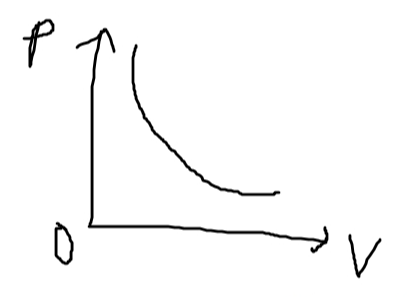
\includegraphics[width=0.3\textwidth]{dang_nhiet.png}
    \caption{Quá trình đẳng nhiệt}
    \label{dang_nhiet}
\end{figure}
ta tính được:
$$A=\int_{V_{1}}^{V_{2}}PdV=\int_{V_{1}}^{V_{2}}\frac{nRT}{V}=nRT \ln{\frac{V_{2}}{V_{1}}}$$
Do $\Delta U=Q-A=0$ nên $Q=A$, vậy ta có:
\begin{tcolorbox}
    Quá trình đẳng nhiệt:
    $$\Delta U=0$$
    $$Q=A=nRT\ln{\frac{V_{2}}{V_{1}}}$$
\end{tcolorbox}
\subsubsection{Quá trình đẳng áp}
Trong quá trình đẳng áp, áp suất của hệ nhiệt động không thay đổi trong cả quá trình nên $\Delta U=nC_{v}\Delta T$, xét đồ thị POV ta tính được:
\begin{figure}
    \centering
    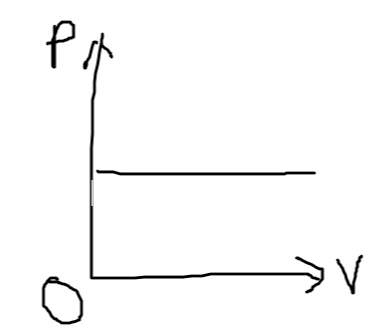
\includegraphics[width=0.3\textwidth]{dang_ap.png}
    \caption{Quá trình đẳng áp}
    \label{dang_ap}
\end{figure}
$$A=\int_{V_{1}}^{V_{2}}PdV=P\Delta V=nR\Delta T$$
Từ phương trình $\Delta U=nC_{v}\Delta T=n\frac{iR}{2}\Delta T=Q-A$, ta tính được:
$$Q=n(\frac{i}{2}+1)R\Delta T=nC_{p}\Delta T$$ Ta đặt $C_{p}=n(\frac{i}{2}+1)R$ và gọi đây là nhiệt dung mol đẳng áp.
\begin{tcolorbox}
    $$\Delta U=nC_{v}\Delta T$$
    $$Q=nC_{p}\Delta T$$
    $$A=nR\Delta T$$
\end{tcolorbox}
\subsubsection{Quá trình đẳng tích}
Trong quá trình này do thể tích của hệ nhiệt động không thay đổi nên $A=0$, hệ không sinh công, ta có:
\begin{tcolorbox}
    $$\Delta U=nC_{v}\Delta T$$
    $$Q=nC_{v}\Delta T$$
    $$A=0$$
\end{tcolorbox}
\subsubsection{Quá trình đoạn nhiệt}
Trong quá trình này hệ nhiệt động không trao đổi nhiệt lượng với môi trường bên ngoài nên $Q=0$, đồ thị POV của quá trình này tương đối đặc biệt do phương trình của nó:
$$P_{1}V_{1}^{\gamma}=P_{2}V_{2}^{\gamma}$$
$$T_{1}V_{1}^{\gamma-1}=T_{2}V_{2}^{\gamma-1}$$
\begin{figure}
    \centering
    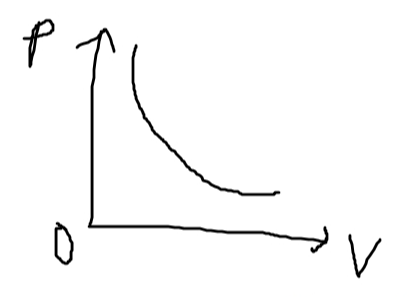
\includegraphics[width=0.3\textwidth]{dang_nhiet.png}
    \caption{Quá trình đoạn nhiệt}
    \label{doan_nhiet}
\end{figure}
Ta có:
\begin{tcolorbox}
    $$\Delta U=nC_{v}\Delta T$$
    $$Q=0$$
    $$A=-nC_{v}\Delta T$$
\end{tcolorbox}
Bài tập:
\\1. Tự xây dựng lại tất cả các công thức đã nắm được ở phần trên.
\\2. Một hệ chứa 5 mol khí Heli giãn nở dưới áp suất không đổi khi nhiệt độ tăng lên 20 độ K.
\begin{itemize}
    \item Tính nhiệt lượng cung cấp cho hệ trong quá trình đó
    \item Tính biến thiên nội năng của hệ
    \item Tính công khí khi thực hiện giãn nở
\end{itemize}
\section{Nguyên lý 2 nhiệt động lực học}
\subsubsection{Động cơ nhiệt và cách phát biểu nguyên lý 2 theo Thomson}
Động cơ nhiệt là 1 trong 2 loại máy nhiệt chính với cơ chế hoạt động là \textbf{nhận nhiệt lượng và sinh công}.
\begin{figure}
    \centering
    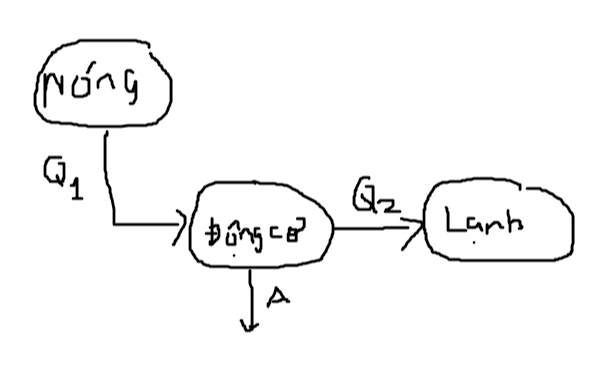
\includegraphics[width=0.8\textwidth]{dongco.png}
    \caption{Động cơ nhiệt}
    \label{dongco}
\end{figure}
\\Động cơ nhiệt nhận nhiệt lượng $Q_{1}$ từ nguồn nóng, chuyển hóa thành công $A$ và một phần năng lượng thất thoát $Q_{2}$ thoát ra từ nguồn lạnh.
\\Vì cơ chế chính của động cơ nhiệt là chuyển hóa lượng nhiệt nhận vào từ nguồn nóng $Q_{1}$ thành công $A$, nên ta có phương trình tính hiệu suất của máy nhiệt:
$$H=\frac{A}{|Q_{1}|}=\frac{|Q_{1}|-|Q_{2}|}{|Q_{1}|}$$
Người ta đã rất cố gắng để giảm thiểu lượng nhiệt thất thoát ra ngoài nguồn lạnh $Q_{2}$ nhưng không thể, kết quả này đã được khái quát hóa thành nguyên lý thứ 2 theo cách phát biểu của Thomson như sau:
\\ \textit{Không tồn tại trong tự nhiên quá trình nào có thể chuyển hóa hoàn toàn nhiệt lượng thành công mà không để lại dấu vết gì cho môi trường xung quanh (không thể chế tạo được động cơ vĩnh cửu loại 2, loại động cơ sinh công bằng đúng năng lượng nhận được)} 
\subsubsection{Máy lạnh và cách phát biểu nguyên lý 2 theo Clausius}
Khác với cơ chế hoạt động của động cơ nhiệt, cơ chế hoạt động của máy lạnh là \textit{tiêu thụ công để vận chuyển nguồn lạnh sang nguồn nóng}.
Máy lạnh nhận công $A$ từ động cơ để lấy nhiệt lượng lạnh $Q_{2}$ từ nguồn lạnh và chuyển nó sang nguồn nóng do \textbf{nhiệt không thể tự chuyển từ nguồn lạnh sang nguồn nóng}.
\begin{figure}
    \centering
    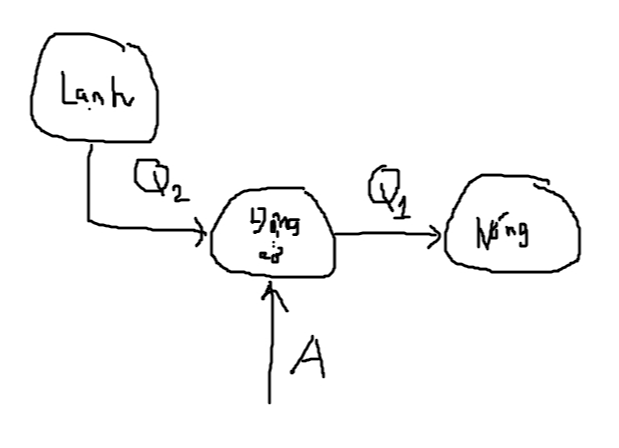
\includegraphics[width=0.8\textwidth]{maylanh.png}
    \caption{Máy lạnh}
    \label{maylanh}
\end{figure}
Vì ta muốn chuyển càng nhiều nhiệt lượng lạnh $Q_{2}$ càng tốt nên ta xây dựng công thức hệ số làm lạnh:
$$K=\frac{|Q_{2}|}{A}=\frac{|Q_{2}|}{|Q_{1}|-|Q_{2}|}$$
Khi $A$ càng nhỏ thì hệ số làm lạnh $K$ càng lớn, hiệu quả làm lạnh càng cao. Trong lịch sử, người ta đã cố gắng đưa $A\to 0$ nhưng đều thất bại. Clausius đã phát biểu nguyên lý 2 như sau:
\\ \textit{Nhiệt không thể tự truyền từ môi trường lạnh hơn sang môi trường nóng hơn, hay nói cách khác là không thể chế tạo máy lạnh vĩnh cửu, loại máy đưa nhiệt lượng từ nguồn lạnh sang nguồn nóng không dùng công}.
Hai cách phát biểu nguyên lý 2 của Thomson và Clausius hoàn toàn tương đương nhau.
\section{Chu trình Carnot}
Chu trình Carnot là một chu trình thuận nghịch đơn giản nhất có khả năng sinh công, đề bài có thể sẽ yêu cầu vẽ và trình bày lại chu trình Carnot. Để đơn giản, ở đây ta chỉ xét chu trình Carnot theo chiều xuôi, tức là chiều của các động cơ nhiệt sử dụng chu trình Carnot.
\begin{figure}
    \centering
    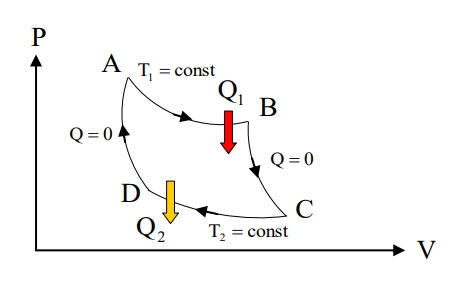
\includegraphics[width=0.8\textwidth]{carnot.png}
    \caption{Minh họa chu trình Carnot}
    \label{carnot}
\end{figure}
Hoạt động của chu trình Carnot rất đơn giản gồm 4 quá trình, 2 quá trình đẳng nhiệt và 2 quá trình đoạn nhiệt xen kẽ nhau
\begin{enumerate}
    \item Từ A đến B, quá trình dãn nở đẳng nhiệt ở nhiệt độ $T_{1}$, áp suất giảm chậm từ $P_{A}$ về $P_{B}$, thể tích tăng nhanh từ $V_{A}$ đến $V_{B}$, hệ nhận nhiệt lượng $Q_{1}$ từ môi trường.
    \item Từ B đến C, quá trình dãn nở đoạn nhiệt ở nhiệt độ $T_{1}$, áp suất giảm nhanh từ $P_{B}$ đến $P_{C}$, thể tích tăng chậm từ $V_{B}$ đến $V_{C}$, nhiệt độ giảm từ $T_{1}$ đến $T_{2}$.
    \item Từ C đến D, quá trình nén khí đẳng nhiệt ở nhiệt độ $T_{2}$, áp suất tăng chậm từ $P_{C}$ về $P_{D}$, thể tích giảm nhanh từ $V_{C}$ đến $V_{D}$, hệ tỏa nhiệt lượng $Q_{2}$ ra môi trường.
    \item Từ D đến A, quá trình nén khí đoạn nhiệt ở nhiệt độ $T_{2}$, áp suất tăng nhanh từ $P_{D}$ đến $P_{A}$, thể tích giảm chậm từ $V_{D}$ đến $V_{A}$, nhiệt độ tăng từ $T_{2}$ về $T_{1}$.
\end{enumerate}
Đối với động cơ nhiệt hoạt động bằng chu trình Carnot, ta cũng có thể dùng công thức tính hiệu suất hoạt động tương tự như trên.
\\Bài tập: Một tủ lạnh dùng công 150J để lấy nhiệt lượng 560J từ buồng lạnh, hãy xác định hệ số làm lạnh của tủ và nhiệt lượng đã tỏa ra môi trường.